\documentclass[tikz,border=10pt]{standalone}
\usepackage{amsmath}
\usepackage{amssymb}

\begin{document}
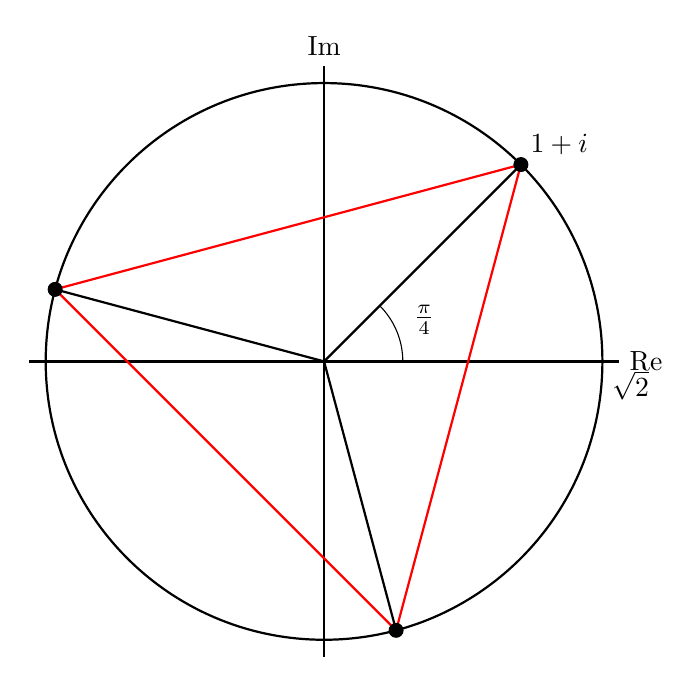
\begin{tikzpicture}[>=stealth, scale=2.5]
    % Draw the axes
    \draw[thick] (-1.5,0) -- (1.5,0) node[right] {Re};
    \draw[thick] (0,-1.5) -- (0,1.5) node[above] {Im};
    
    % Draw the circle with radius sqrt(2)
    % We use 1.414 for the radius in coordinates
    \draw[thick] (0,0) circle (1.414);
    
    % Define the roots (Angles: 45, 165, 285)
    \coordinate (Z0) at (45:1.414);
    \coordinate (Z1) at (165:1.414);
    \coordinate (Z2) at (285:1.414);
    
    % Draw the lines from origin to roots
    \draw[thick] (0,0) -- (Z0);
    \draw[thick] (0,0) -- (Z1);
    \draw[thick] (0,0) -- (Z2);
    
    % Draw the red triangle connecting the roots
    \draw[red, thick] (Z0) -- (Z1) -- (Z2) -- cycle;
    
    % Draw the dots at the vertices
    \filldraw (Z0) circle (1pt) node[above right] {$1+i$};
    \filldraw (Z1) circle (1pt);
    \filldraw (Z2) circle (1pt);
    
    % Label the radius on the x-axis
    \node[below right] at (1.414,0) {$\sqrt{2}$};
    
    % Draw the angle arc for pi/4
    \draw (0.4,0) arc (0:45:0.4);
    \node at (22.5:0.55) {$\frac{\pi}{4}$};
    
\end{tikzpicture}
\end{document}
